\chapter{Vicon and Gait Analysis Software Package}
\label{chap:software}
\section{Introduction}

The presented software packages were developed with the help of Alek Lewis and Alex Tacescu, who contributed to the debugging, testing, and ideas to the structure of the packages. This work was published in the journal of Computer Methods and Programs in Biomedicine \cite{goldfarb2021open}. The Vicon \footnote{Vicon, 7388 S. Revere Parkway Suite 901 Centennial CO 80112USA} motion capture system collects a rich set of data for analysis and manipulation. However, the richness of this data set makes the raw data challenging to extract and handle. To handle this data, it was necessary to develop a toolkit to parse the data into data structures that expose the data to other APIs for manipulation and analysis. 

The Vicon motion capture system is a popular motion capture system. This mocap system can export the data in several formats, including C3D \footnote{https://www.c3d.org/}  files and ASCII files. Vicon offers Python and Matlab packages to post-process the data; these packages only work on a computer with an active Vicon Nexus software package, making it challenging to work with the data. 

C3D files contain rich data that can be imported by popular biomechanical systems such as OpenSim \cite{seth2018opensim}. OpenSim will ingest the data and build an analysis model. The Biomechanical Toolkit offers a powerful tool for handling the raw C3D files to allow researchers to work with the mocap data and apply methods and algorithms \cite{barre2014biomechanical}. This package is written in C++, a compiled language, not an interpreted language. The advantage of an interpreted language like Python is that it is easier to implement, and code can be executed on the fly. This is in contrast to C++ which has complex syntax with better computation performance \cite{varisteas2018distributed} \cite{bargiacchi2020ai}. Computational time is less of a concern when analyzing data, where a priority is more focused on obtaining results and extracting information than real-time functionality. The toolkit developed at Cleveland State University gait lab is an open-source tool for analyzing mocap data  \cite{DTK2014} \cite{GATK2014}. While this package was developed in Python, this tool lacks flexibility and modularity. The complexity of the toolkit makes it difficult to separate marker trajectories and handle marker analysis from gait data.   

A new toolkit was developed to manipulate and analyze Vicon and Gait data to solve these problems. Three software packages are presented; the Gait Core package, the Vicon Toolkit Package, and the Gait Analysis Toolkit Package. The software packages separate the tools for handling the Vicon marker data and the tools for gait analysis. This structure, shown in \autoref{fig:software}, allows for each software package to be used as stand-alone or in a unified system. The GaitCore package allows for a standard API to be used along with constant data types.   

The three software packages are: 
 \textbf{GaitCore}\footnote{https://github.com/WPI-AIM/AIM\_GaitCore}, \textbf{Vicon toolkit}\footnote{https://github.com/WPI-AIM/AIM\_Vicon},  \textbf{Gait Analysis toolkit}\footnote{https://github.com/WPI-AIM/AIM\_GaitAnalysisToolkit} as described in \autoref{fig:software}; this was done to abstract the functionality and use it for different applications and mocap systems. The GaitCore package contains the low-level APIs that build the data structures. The Vicon package contains APIs to parse and manipulate the raw mocap data. The Gait Analysis toolkit provides high-level APIs to analyze gait trajectories and use them to build motion models. 

The advantage of these packages over similar packages is the underlining structure and modularity. This codebase can be extended to handle other mocap systems, which would have access to the built-in computation and analytical tools discussed below. The interpreted language also allows the researcher not familiar with C++ to quickly access and analyze their data. The critical functionality of the package is detailed below. The methods and algorithms used to build the package are also described. 




\begin{figure}[hbt]
    \centering
    \includegraphics[scale=0.15]{images/software/software.png}
    \caption[Software Architecture]{Software architecture of the Vicon-specific toolkit for importing and processing data, the Gait Toolkit for motion analysis which is not specific only to Vicon, the GaitCore structure, and user applications.}
    \label{fig:software}
\end{figure}


\section{GaitCore}
At the center of our Vicon and Gait Analysis tool kit libraries is the GaitCore package. The GaitCore package provides low-level objects used in the Vicon and Gait Analysis Toolkit packages. This package allows the data to be manipulated and stored for consistent structures and readability.

The GaitCore package objects provide APIs to initialize the object and work with the data. Each class has override operators to allow for mathematical operations to be performed. The objects in the GaitCore package are the following:

\begin{itemize}[noitemsep]
\item \textbf{Core}:
\begin{itemize}[noitemsep]
    \item \underline{Point}: Holds a 3D point $(x,y,z)$, there are override operators and functions to perform basic vector operations. It can also be converted into a numpy array to perform more advanced operations.
    \item \underline{PointArray}: Holds a list of Point objects. This class provides functions to access to $X$, $Y$, and $Z$ axis. 
    \item \underline{Newton}: Holds angle, power, torque, force information that is calculated by the Nexus system. 
    \item \underline{Data}: Holds time sequenced data, it can be used to organize joint data against the time period. This class has two fields; data and time. It is a method of sequencing the data.  
\end{itemize}
\item \textbf{Bio}:
\begin{itemize}
    \item \underline{Joint}: Holds information on a single joint
    \item \underline{Leg}: Holds three joints (hip, knee, ankle)
    \item \underline{Arm}: Holds three joints (shoulder, elbow, wrist)
    \item \underline{Trunk}: Holds four joints (head, spine, thorax, plevis)
    \item \underline{Side}: Holds left and right side of the body
\end{itemize}
\end{itemize}




\section{Vicon Package}
\subsection{Overview}
The Vicon Toolkit Package parses and organizes the data exported by the Vicon Nexus software. The Nexus software exports an ASCII file with headers distributed throughout the row of the file. The Vicon parser extends an abstract base class \textit{Mocap}; this allows for an abstract of the core functionality required for different mocap systems, which includes the marker interpolation and joint modeling and allows the tools discussed to be used for other mocap systems such as the Optitrack \footnote{Optitrack, NaturalPoint, Inc. Corvallis, OR 97339}.  
 The tools in this package are summarized below: 

\begin{itemize}[noitemsep]
    \item Gap filling of missing data 
    \item Organizing the data from the plug-in gait model 
    \item Sorting of rigid bodies
    \item Access to force plates and EMGs 
\end{itemize}


Our Vicon Toolkit Package sorts the data into three buckets (classes): markers, devices, and model outputs. Each of these classes has internal functions for analysis. The classes were created to align the section headers in the ASCII file export from Vicon Nexus. 

The Vicon object is initialized with a single line of code. The only mandatory parameter is the path to the ASCII file; there are optional parameters for gap filling and interpolation of missing data. The interpolated data can be exported to a new file for later use.  \autoref{setup} shows how to initialize the Vicon object.

\lstinputlisting[language=Python, 
caption=This block shows how to initialize the Vicon object and use the interpolation parameters, label=setup]{code/set_up.py}


\subsection{Gap Filling}

A common complication during a mocap trial is that the cameras will lose track of one or several markers; this results in gaps in the data. The Vicon Nexus software provides several tools to pattern and spline fill missing marker data, filling most gaps. However, some gaps might remain in the exported data. These gaps need to be filled in before any analysis can be performed. Tools were built into the package to fill in and interpolate missing data. The tools are abstracted for the implementation and development of custom interpolation methods. The Vicon object will keep track of which values were interpolated so that the user of this package can track what data was interpolated. 


There has been substantial effort to research and develop missing marker interpolation methods. Each method is designed under different constraints and is optimized for different scenarios, including but not limited to biomechanical research. These methods vary from simple spline fitting to complicated statistical methods. 

Akima spline interpolation \cite{wang2014real} is a simple polynomial interpolation method. The Akima method uses $3^{rd}$ order continuously differentiable polynomial. The Akima's feature method's feature is that it has a continuous $1^{st}$  order derivative through its endpoints and behaves well when the second derivative of the data is rapidly changing. \autoref{eq:akima} defines the the polynomial between the two points $(x_{1}, y_{1})$ and $(x_{2}, y_{2})$, with slopes $t_{1}$ and $t_{2}$ respectively. The Akma method is limited in several ways; it assumes that a polynomial can interpret the marker's movement. It does not consider the marker's velocity vector and the movement of other markers attached to the same body. 

\begin{equation} \label{eq:akima}
\large
\begin{split}
        y &= p_{0} + p_{1}(x - x_{1}) + p_{2}(x - x_{1})^{2} + p_{3}(x - x_{1})^{3} \\
        where, \\
          p_{0} &= y_{1} \\
    p_{1} &= t_{1} \\
    p_{2} &= (3(y_{2} - y_{1})/(x_{2} - x_{1}) - 2t_{1} - t_{2})/(x_{2} - x_{1}) \\
    p_{3} &= (t_{1} + t_{2} - 2(y_{2} - y_{1})/(x_{2} - x_{1}))/(x_{2} - x_{1})^{2}
\end{split}
\end{equation}

Piaze \textit{et. al} attempting to resolve some of the limitations of pure interpolation by considering the velocity vector of the marker and its recent history \cite{piazza2009towards}. This method assumes that a marker will move locally in a straight line or a circle pattern. A backlog of markers is stored to find the forward vector of motion; this backlog is used to estimate a marker's velocity. A local marker model can be found and used to interpolate to find small gaps in the marker's trajectory using both the linear and angular velocity. This method is relatively simple in its implementation and execution. It takes advantage of the marker's prior motion to interpolate its future position and does not require the marker noise variance model. This method has several limitations; it only relies on a single marker, meaning that it cannot infer a marker's position from other markers. In addition, it assumes that all motion on a body can either be modeled as linear or circular, which may not always be the case. The velocity is also calculated by examining the backlog of the marker's location, while this leads to a vector being less subject to noise from frame to frame. It can lead to the velocity vector lagging behind the motion of the marker. 

McCain \textit{et. al} proposed a method that takes advantage of rigid bones in the human body, and the marker attached to the bones will have the same relative motion \cite{li2010bolero}. In this method, a hard and soft assignment method was examined. The soft assignment method relaxes some of the assumptions of marker noise caused by skin movement. This method is based on the expectation-maximization (EM) algorithm and Kalman-like filtering method; this is a statistical-based method that requires knowledge of the marker noise and additional markers to work properly. 

A similar method was developed by Lasenby \textit{et. al}, this method also used a bone constraint method \cite{aristidou2013real}. However, this method did not constrain its movement to be linear; it replaced the linear Kalman filter with an unscented Kalman filter. An unscented Kalman filter allows for nonlinear models of the motion to be assumed. This method takes full advantage of the markers attached to a rigid bone structure. It also uses a variable tune model with a target velocity and acceleration of the markers. The latter, however, is subject to too much noise to be computationally useful. This method requires three markers per body for tracking; these markers allow the marker to calculate the body's 3D location in space. While this number of markers would be common for biomechanical trials, it requires many markers to be used; this makes it unsuitable for trials with few markers or markers not attached to rigid bodies.

Each of the methods discussed above is optimal for different applications and research. Furthermore, new methods can be developed to produce better results or suit a particular application or research. The package was built so that the user could specify the desired interpolation method; this is unique compared to other packages. To the best of our knowledge, other packages either do not offer an interpolation method, or the method is fixed.  

\subsection{Rigid Bodies}

Rigid bodies in mocap are built from a collection of individual markers on a body segment. Three or more markers are required to define the position and orientation of the body in space, allowing for the relative pose of the body to be found in all the frames. The marker placement can be set \footnote{https://www.vicon.com/hardware/accessories/} using rigid plates with known marker position. These rigid plates are strapped to the person's body to record the positions of the body. \autoref{fig:markers_side} shows the coordinate frames on the leg of a person. \autoref{fig:rigidbody} shows the rigid body plate with marker locations. 

\begin{figure}
\centering 
\begin{subfigure}{0.4\linewidth} 
  \centering 
  \includegraphics[scale=0.05,frame]{images/software/marker_side_coor.png} 
  \caption[RigidBody Frames]{Rigid Body Frames on the Leg} 
  \label{fig:markers_side} 
\end{subfigure} 
%
\begin{subfigure}{0.4\linewidth} 
  \centering 
    \centering
    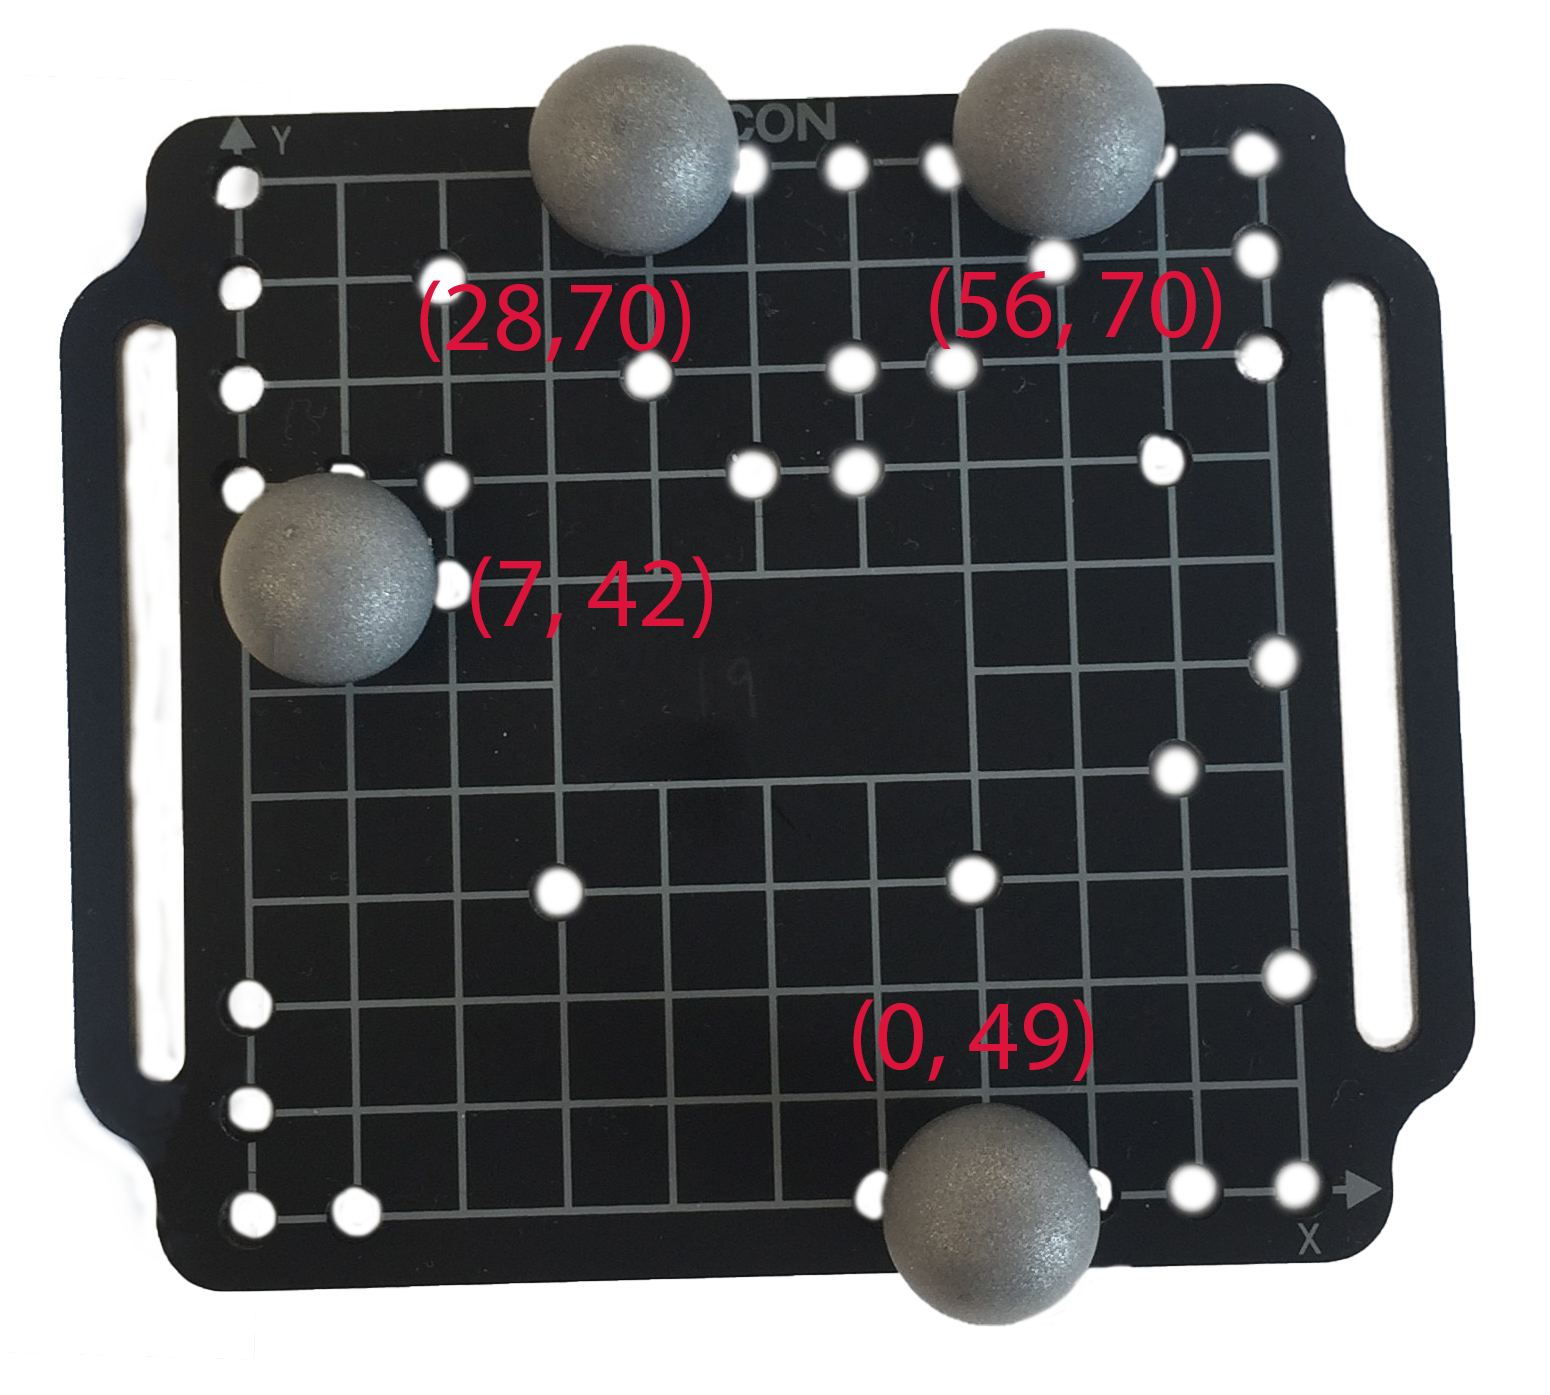
\includegraphics[scale=0.11]{images/software/rigidbody_label.png} 
    \caption{Labeled rigid body plate from Vicon}
    \label{fig:rigidbody}
\end{subfigure} 
\caption[Rigidbodies and Placement]{Rigid Bodies and Placement} 
\label{fig:markers} 

\end{figure} 

A least-squares method is used for the transformation between the markers point cloud \cite{arun1987least}. This method requires the relative location of the markers, which is set using rigid body plates. This is described in \autoref{eq:pointcloudtransformation}. In this equation, $A$ and $B$ are the recorded locations of all the markers in different frames. The goal is to calculate the translation $t$ and rotation $R$ between the two point clouds. The rotation is found using Singular value decomposition (SVD). \autoref{eq:rotationPointclouds} is used to find the rotation. To isolate the translation component- the marker point clouds are re-centered around the origin by subtracting the centroid (\autoref{eq:centroid}) of the point cloud. Here, $A_i$ and $B_i$ is a $3x1$ vector of the position ($[x,y,z]$) of a single marker. Using the rotation matrix $R$ the translation is then computed using  \autoref{eq:translationPointclouds}.  The error for every transformation is calculated and returned; it is used to evaluate the transformation's goodness of fit. \autoref{eq:errorPointclouds} is used to calculate the fit error.   


\begin{equation}
    \large
    RA + t = B
    \caption{Marker point cloud transformation}
    \label{eq:pointcloudtransformation}
\end{equation}

\begin{equation}
\large
    centroid_{A,B} &= \frac{1}{N} \sum_{i}^{N} \{A,B\}_i 
    \caption{Calculation of the pointcloud centroid}
    \label{eq:centroid}
\end{equation}


\begin{equation}
\large
    \begin{split}
        H &= ( A - centroid_A) ( B - centroid_B) ^T\\
    [U,S,V] &= SVD(H)\\
    R &= VU^T    
    \end{split}
    \caption{Finding the rotation matrix between the marker pointclouds}
    \label{eq:rotationPointclouds}
\end{equation}
    
\begin{equation}
    \large
    t = centroid_B - R \times centroid_A
    \caption{Marker point cloud transformation}
    \label{eq:translationPointclouds}
\end{equation}

\begin{equation}
    \large
    err = \sum_{i}^{N} || RA_i + t -B_i ||^2
    \caption{Error of the point cloud fitting}
    \label{eq:errorPointclouds}
\end{equation}


The Vicon toolkit will automatically gather markers into rigid bodies and produce a transformation matrix for each rigid body for every point in the trial. The transformation is used to locate relative movement between the various bodies. The novelty of this package is its flexibility to generate rigid bodies from a set of markers. Due to the abstraction layer, it can be used for any mocap system. 


% \subsection{Addition Features}

\subsection{Model Outputs}
The Vicon Nexus software available from Vicon has several plug-in models (upper and lower) for fitting marker data to the human body. The plug-in models are used to calculate the joint angle, torque, power, and force output, and these values are critical for the analysis of gaits and human motion. The Vicon package stores all of this data in the Newton class. The joint class stores the data for a single joint, such as the hip, shoulder, or knee. This structure allows for easy access to the joint kinematics and dynamics. \autoref{modeloutput} shows how to get the left hip angle of a subject while walking. In the above-referenced code, if the angle operator is replaced with "moment," the torque around the joint can be accessed. 


\lstinputlisting[language=Python, 
caption=This block shows how to get the hip angle around the $X$ axis of the course of the entire trial, label=modeloutput]{code/modeloutput.py}

This package provides single-line access to all the model output information. The joint trajectories of the gait cycle can be studied and used for developing motion models using the model output information. All the critical information is provided to the user.  



\subsection{Visualization of Trial}
The \textit{play()} function generates a 3D plot of every marker position through time. \autoref{fig:playFigure} show a frame from the \textit{play()} from a trial where a subject climbed a staircase. Markers and rigid bodies were placed on the subject's legs, and a rigid body was placed on each of the staircase steps to locate each step. The Vicon object also has a graphing method that will create and plot a selected field graph.

\begin{figure}
    \centering
    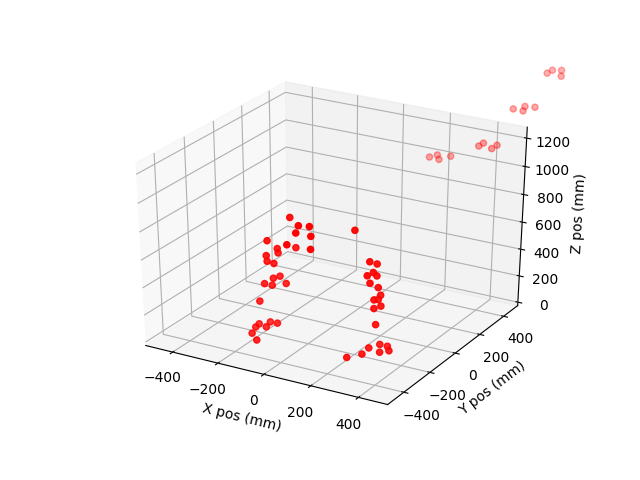
\includegraphics[scale=0.6]{images/software/play.png}
   \caption[Play Demonstration]{Marker locations in a single frame during a trial of climbing stairs. Each of the red dots is a marker. The marker clusters on the right hand side are rigid bodies placed on each stair. }
    \label{fig:playFigure}
\end{figure}

\subsection{Joint Calibration}
Locating joints is an important part of analyzing human motion capture data. There are two main types of joints in the human body; ball joints and hinge joints. Hips and ankle are typically modeled as ball joints that have a center of rotation (\textit{CoR}), and while knee joints are very complex with multiple degrees of freedom, they can be simplified to hinge joints \cite{hefzy1996review}, however, this is not ideal. Hinge joint rotate about an axis of rotation (\textit{AoR}) each point on the axis is a CoR \cite{halvorsen1999new}. A method presented by Hiniduma \textit{et. al} use several markers and successive frames to estimation the \textit{CoR} and \textit{AoR} of the model joints. The method of calculating the \textit{CoR} and \textit{AoR} is shown in \autoref{eq:CoR}, where $\overline{(v^p)^n} = 1/N \sum_{k=1}^N (v_k^p)^n$. For reference, when $n=2$, will $v$ be a scalar, and when $n=3$  will $v$ be a vector. Additionally, $p$ represents a marker in the frame, and $k$ is the current frame number. The \textit{AoR} is the Eigenvector corresponding to the minimum Eigenvalue.

\begin{equation}
    \begin{aligned}
        A &= 2 \sum^{P}_{p=1} \Bigg[ \bigg\{  \frac{1}{N} \sum^{N}_{k=1} v_k^p (v_k^p)^T \bigg\} -  \overline{v^p}(\overline{v^p})^T \Bigg] \\
        b &= \sum^{P}_{p=1} \Big[ \overline{(v^p)^3} - \overline{v^p} (\overline{(v^p)^2)} \Big] \\
        CoR &= A \backslash b\\
        AoR &=  eigenVector(A)
\end{aligned}
        \label{eq:CoR}
\end{equation}

A problem with the method above is that the \textit{AoR} has infinite \textit{CoR}, which is not ideal. Since the true center of rotation should be within the constraints of the rigid bodies rotating about the axis. This method can be improved by using a Sequential Least-Squares Programming method to calculate the correct CoR along the axis \cite{Least-Squares-Fitting}. This method worked by finding the minimum distance between a point on the leg and the axis of the joint. The objective function and constraints are shown in \autoref{eq:min}. The parameters were point(s)($p_i$) , the \textit{AoR} ($axis$), and the \textit{CoR}. The objective was to find the minimum distance between the center of mass of the two bodies along the \textit{AoR}. 

The effects of the optimization method are illustrated in \autoref{fig:KneeLocation}, which shows a mocap frame of a person with lower body markers. Each of the red dots is a mark, and the blue dot and line are the \textit{CoR} and \textit{AoR} respectively. \autoref{fig:BadKnee} shows the location of the \textit{CoR} without the optimization, which appears outside the thigh and shank marker clusters. \autoref{fig:GoodKnee} shows the location of the \textit{CoR} with the optimization, which appears inside the thigh and shank marker clusters.



\begin{figure}[]
    \centering
    \begin{subfigure}{.45\textwidth}
        \centering
        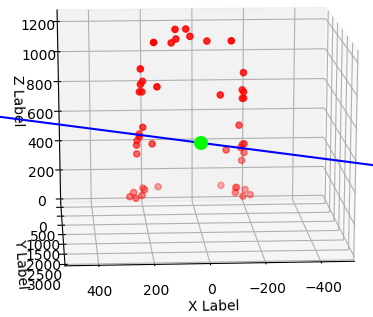
\includegraphics[scale=0.40]{images/software/bad_knee_edit.png}
        \caption[Incorrect Knee Location]{Incorrect Knee Location with out the optimization step}
        \label{fig:BadKnee}
    \end{subfigure}%
    \hfill
    \begin{subfigure}{.45\textwidth}
        \centering
        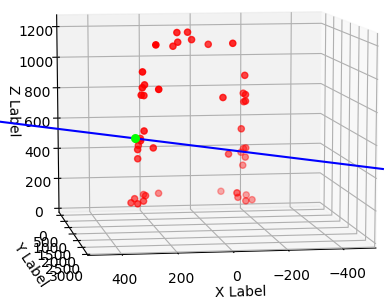
\includegraphics[scale=0.40]{images/software/good_knee_edit.png}
        \caption[Correct Knee Location]{Correct Knee Location using optimization method}
        \label{fig:GoodKnee}
    \end{subfigure}
    \caption[Finding Knee location]{Finding Knee Location. The blue dot is the \textit{CoR}, red dots are marker}
    \label{fig:KneeLocation}
\end{figure}

\begin{equation}
    \begin{aligned}
        x &= \begin{bmatrix} x_1 & x_2  & x_3 & x_4 \end{bmatrix} \\
        min f(p,x) &= \sum_{n=0}^{N} \big[(p_{i}^x - x_1)^2 + (p_{i}^y - x_2)^2 +(p_{i}^z - x_3)^2 \big]^{0.5}     \\
        g(x) &= \begin{bmatrix} x_1 & x_2  & x_3 \end{bmatrix}^T -\hat{x}_{initial} - x_4 (axis) 
    \end{aligned}
    \caption{Minimize the center, p_i represents a point, and $axis$ is line to search along }
    \label{eq:min}
\end{equation}


\section{Gait Analysis Package}

\subsection{Overview}
While the Vicon package provides comprehensive tools to handle the mocap data, the Gait Analysis Toolkit provides more focused tools to handle gait analysis. This package includes: 
\begin{itemize}[noitemsep]
    \item Separating gait cycles
    \item Comparing different subjects gaits
    \item EMG filtering
    \item Learning of gait trajectories
\end{itemize}

The presented tools were developed to compare the gait motion collected during the trial. The toolkit will separate the gait motions into individual gait cycles. The gait cycles can be compared within the trial or against other trials or subjects, allowing for features of the trajectory to be compared to find patterns. 

\subsection{Gait Detection}
\autoref{fig:gaitDetection} show the extract gait cycles. It analyzes the first and second derivatives to find the max peaks and inflection points. This joint angle method can lead to a slight phase shift in a gait cycle; this can be improved using information from the force plates. Once the index of all the gait cycles is found, the devices and model data associated with the gait trail are separated by the indices. Each of the lines is a gait cycle extracted from a separate subject. The start and endpoints of each step should be approximately the same value after the first step; the start and endpoints may vary slightly. 

\begin{figure}[h]
  \centering
    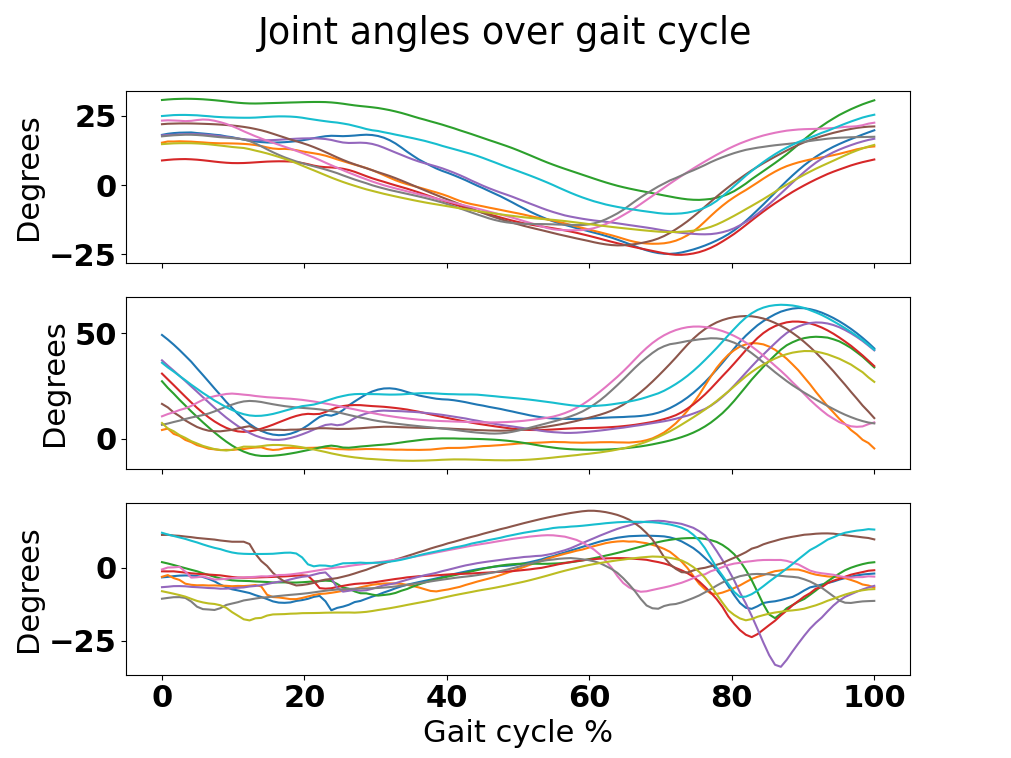
\includegraphics[scale=0.5]{images/software/gaitcycle.png}
    \caption[Gait Cycles]{The joint angle during a gait cycle. Each line represents a different subjects gait. The trajectories were re-sampled to be the same length}
    \label{fig:gaitDetection}
\end{figure}



\subsection{Learning from Demonstration}

The LfD algorithms are built in this package to learn the record biomechanical information; this allows for seemly flow from data collection to replication. \autoref{fig:flowchart} shows a flowchart of how a trajectory is learned. \autoref{fig:learned} shows learned demonstrations and the learned trajectory. The software is based on the other open-source packages \cite{calinon2016tutorial}. While performing the mathematical operations, these other packages are difficult to use outside their provided data set with the codebase. 


\begin{figure}[h!]
    \begin{subfigure}{0.4\linewidth} 
        \centering
        \captionsetup{justification=centering}
        \centerline{
        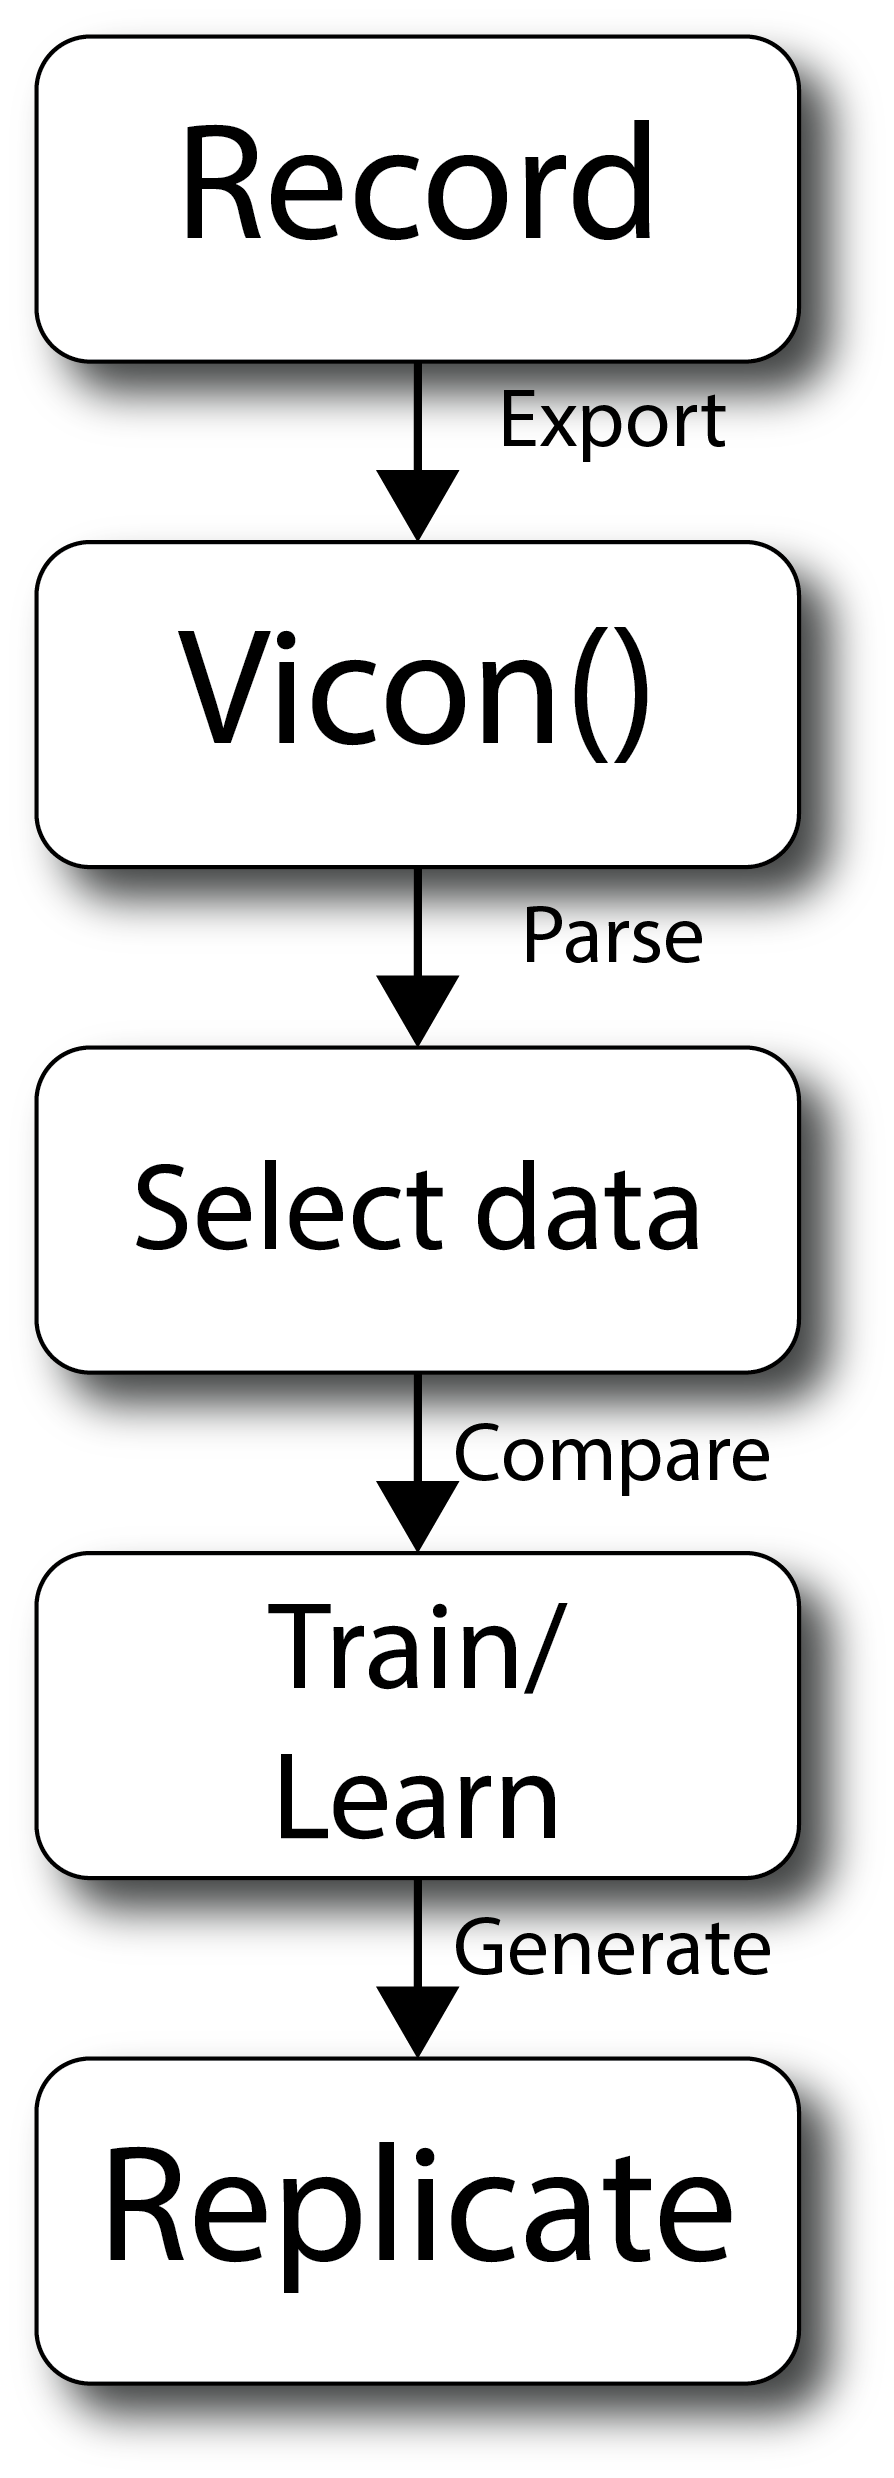
\includegraphics[scale=0.25]{images/software/software_layers.png}}
        \caption{Learning flow chart}
        \label{fig:flowchart}
    \end{subfigure}
    %
    \begin{subfigure}{0.4\linewidth} 
        \centering
        \captionsetup{justification=centering}
        \centerline{
        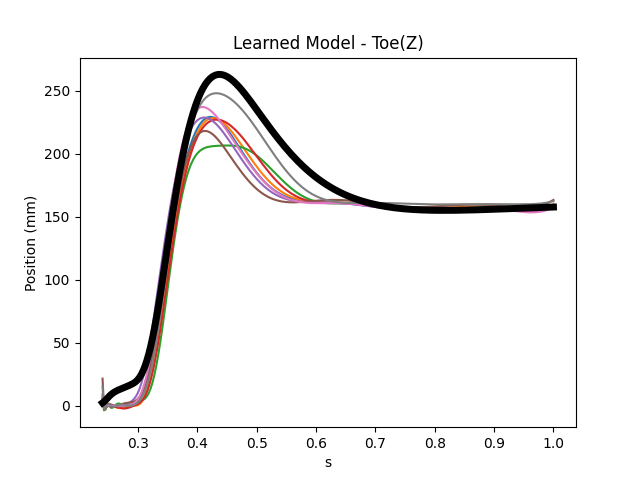
\includegraphics[scale=0.50]{images/software/learnedZ.png}}
        \caption{The thick line is the learned trajectories. The thin lines are the demonstrations that were used to train the model. This model was trained to replicate the toe marker}
        \label{fig:learned}
    \end{subfigure}
    \label{fig:LFDexample}
\end{figure}


DTW (\autoref{eq:DTW}) does not produce smooth trajectories. The trajectories must be smoothed so the derivative of the trajectory is continuous. The smoothed trajectory and its derivative are required to calculate the force model to pull the system along the desired motion. The force model is calculated using \autoref{eq:forcingfunction}, where $x$ is the demonstration trajectory, and $K_p$ and $K_v$ are gains; this is essentially a mass-spring-dampener model. A polynomial to the temporally scaled demonstrations produces smooth, continuous, and differentiable trajectories; this is important when differentiating the demonstrations for encoding the motion model.  \autoref{fig:DTWSmoothing} shows an example of the smoothing and affects the reproduction of the trajectory; this can be seen in \autoref{fig:smoothingcomparison}. As shown in \autoref{fig:unsmoothreplication} when the DTW trajectories are not smoothed, the model cannot replicate the motion. The forcing function shown in blue was calculated using \autoref{eq:forcingfunction}, as shown in the training forcing functions chatter. The chattering is caused by the DTW trajectories having discontinuities that are magnified when the derivative of the signal is taken.  \autoref{fig:smoothreplication} was generated when the smoothing was applied to the trajectories, which resulted in the forcing function being smooth, making it possible to replicate the trajectory more accurately. The smoothed path method as a metric of imitation cost 1,224, while the unsmoothed path method has a cost of 1,890.3, which is approximately a 54.4\% increase in the metric of imitation. 

\begin{equation}
    \Large
    \tau = x + \frac{Kv}{Kp} \dot{x} + \frac{1}{Kp} \ddot{x}
    \caption[Force Term]{Forcing Term}
    \label{eq:forcingfunction}
\end{equation}


\begin{figure}
    \centering
    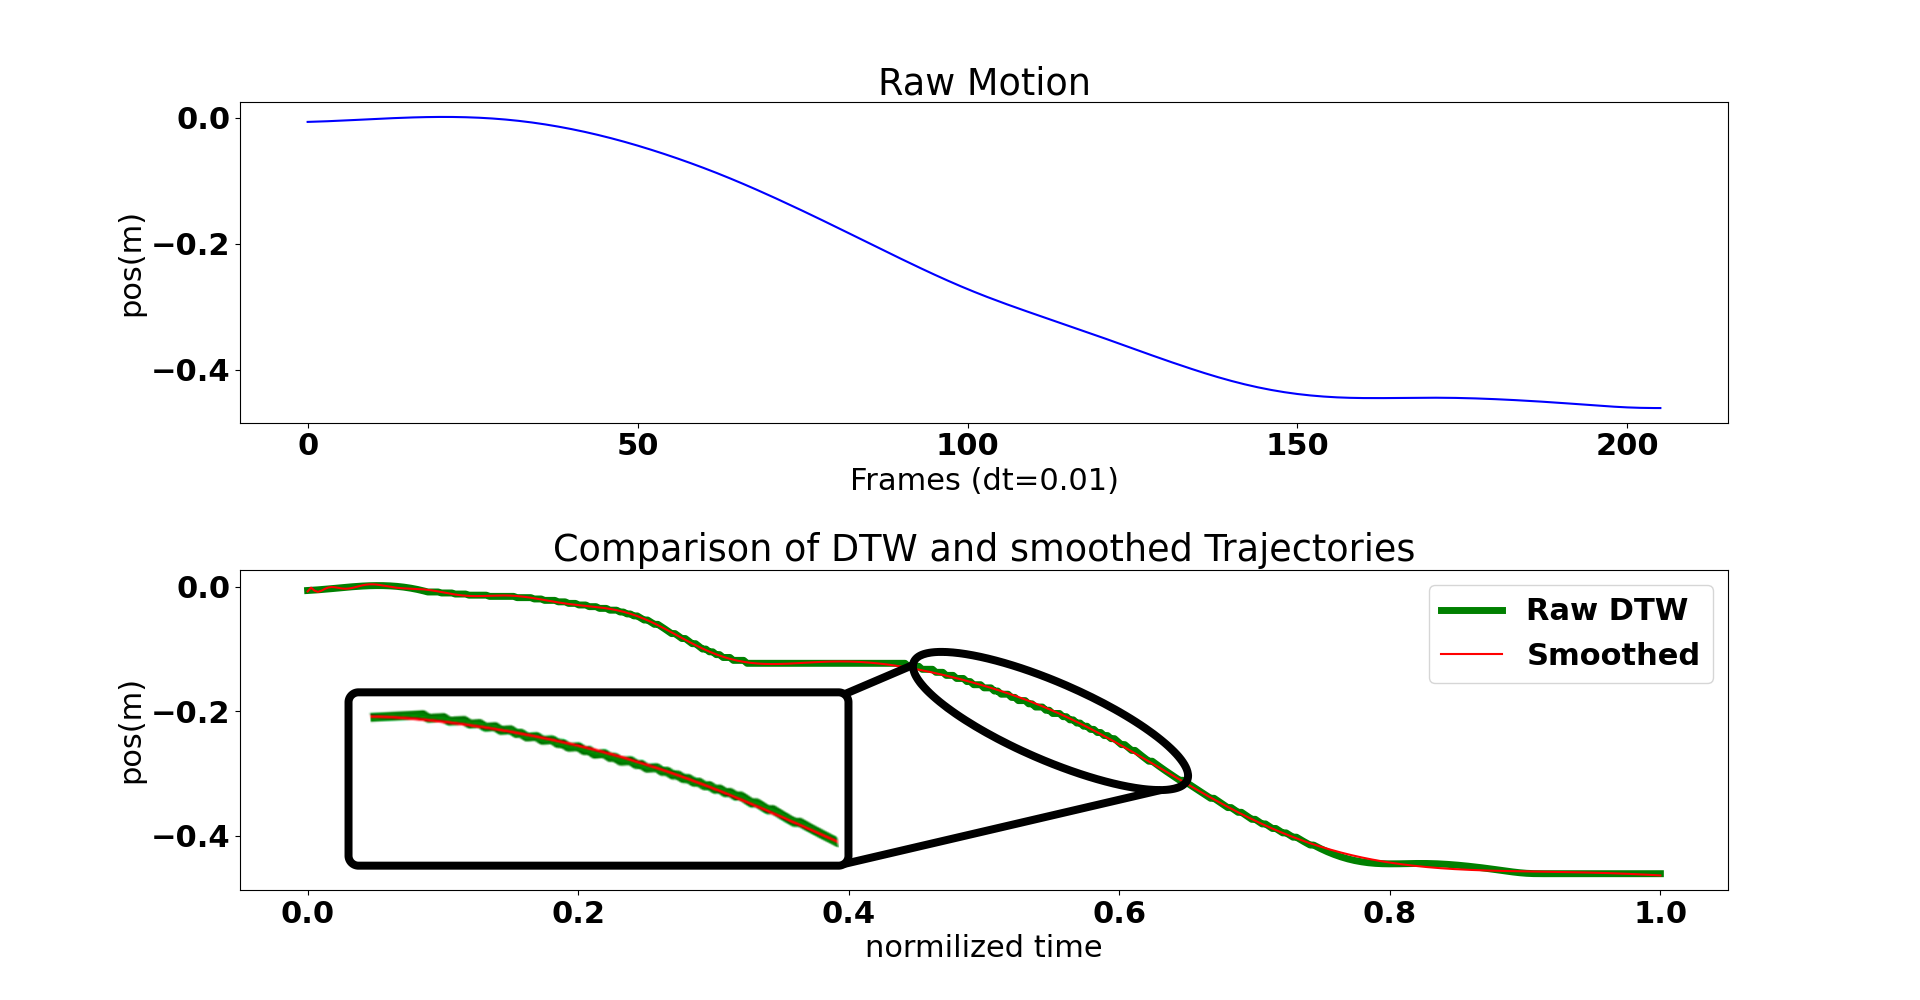
\includegraphics[width=\textwidth]{images/software/DTWsmoothing_annotanted.png}
    \caption[DTW Smoothing]{Using Polynomials to smooth the DTW trajectory. The chatter can be seen in the enlarged box.}
    \label{fig:DTWSmoothing}
\end{figure}



\begin{figure}[h!]
    \begin{subfigure}{\textwidth} 
        \centering
        \captionsetup{justification=centering}
        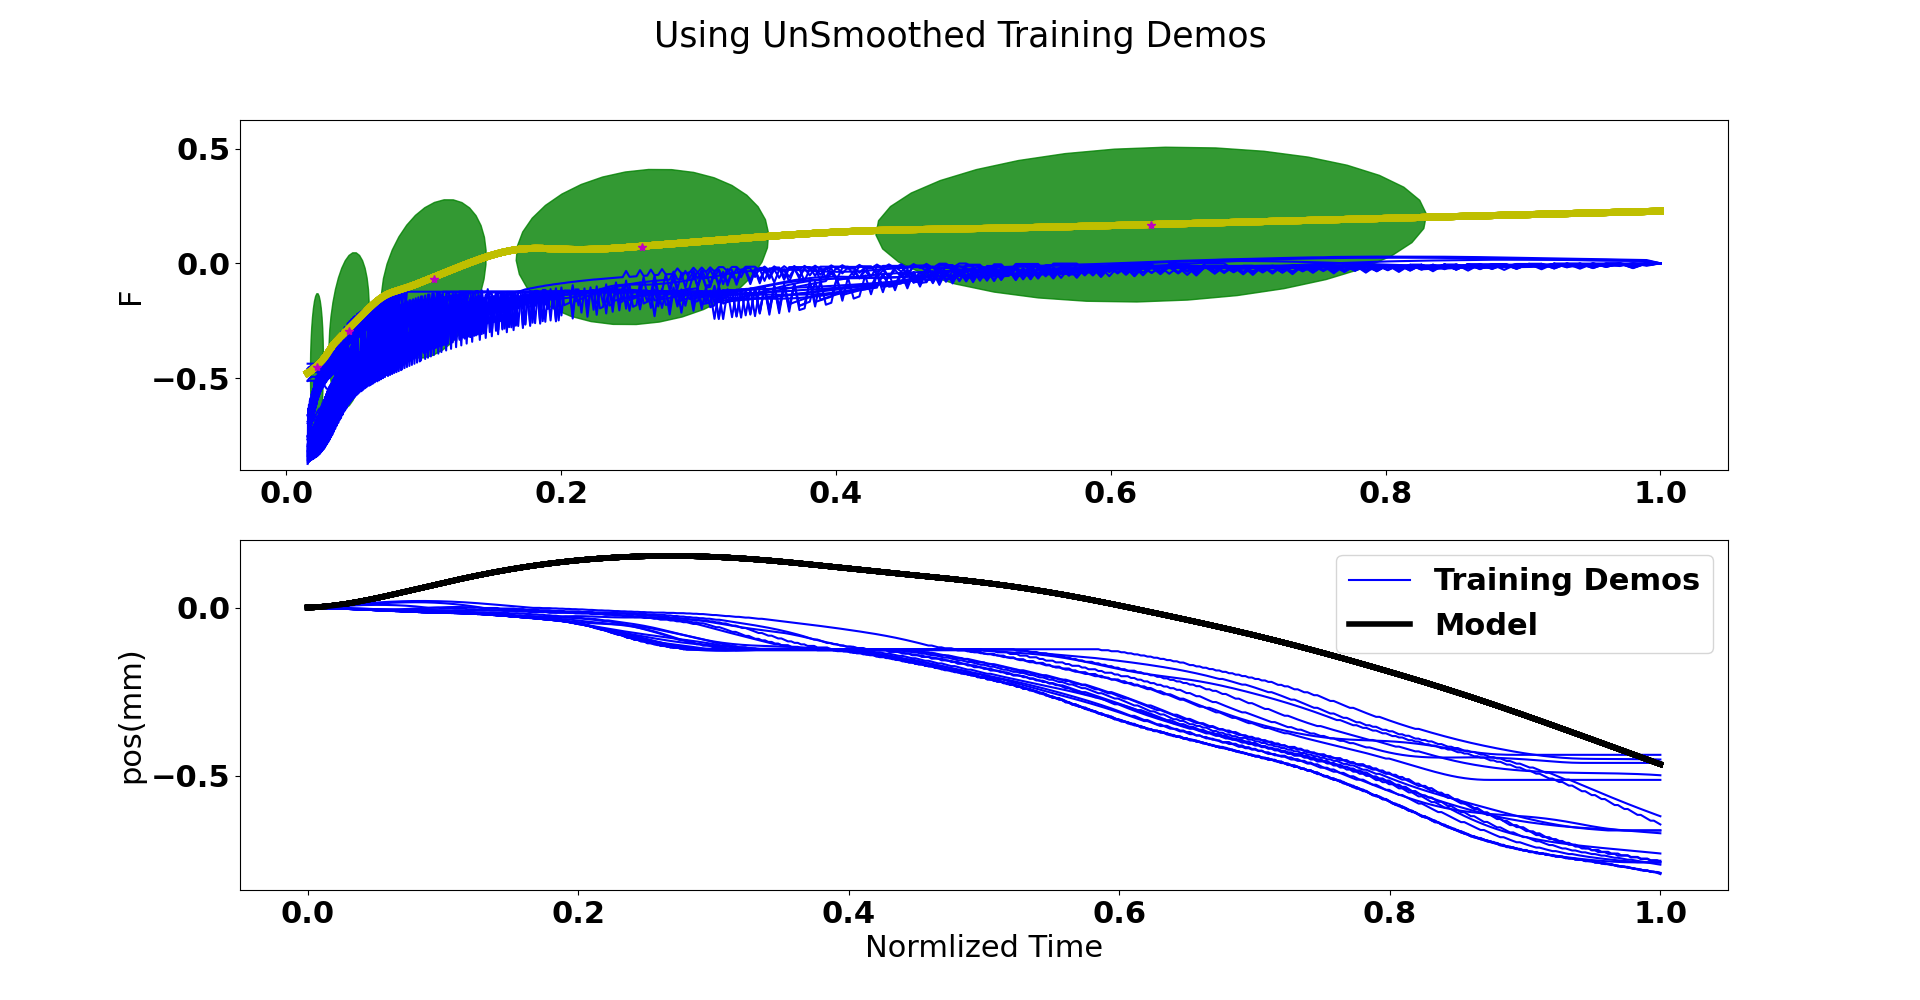
\includegraphics[width=\textwidth]{images/software/unsmoothed_repruction.png}
        \caption{Forcing function and replicated trajectory. As shown the model was not able to follow the desired motion and the forcing functions have chattering along the motion.}
        \label{fig:unsmoothreplication}
    \end{subfigure}
      \begin{subfigure}{\textwidth} 
        \centering
        \captionsetup{justification=centering}
        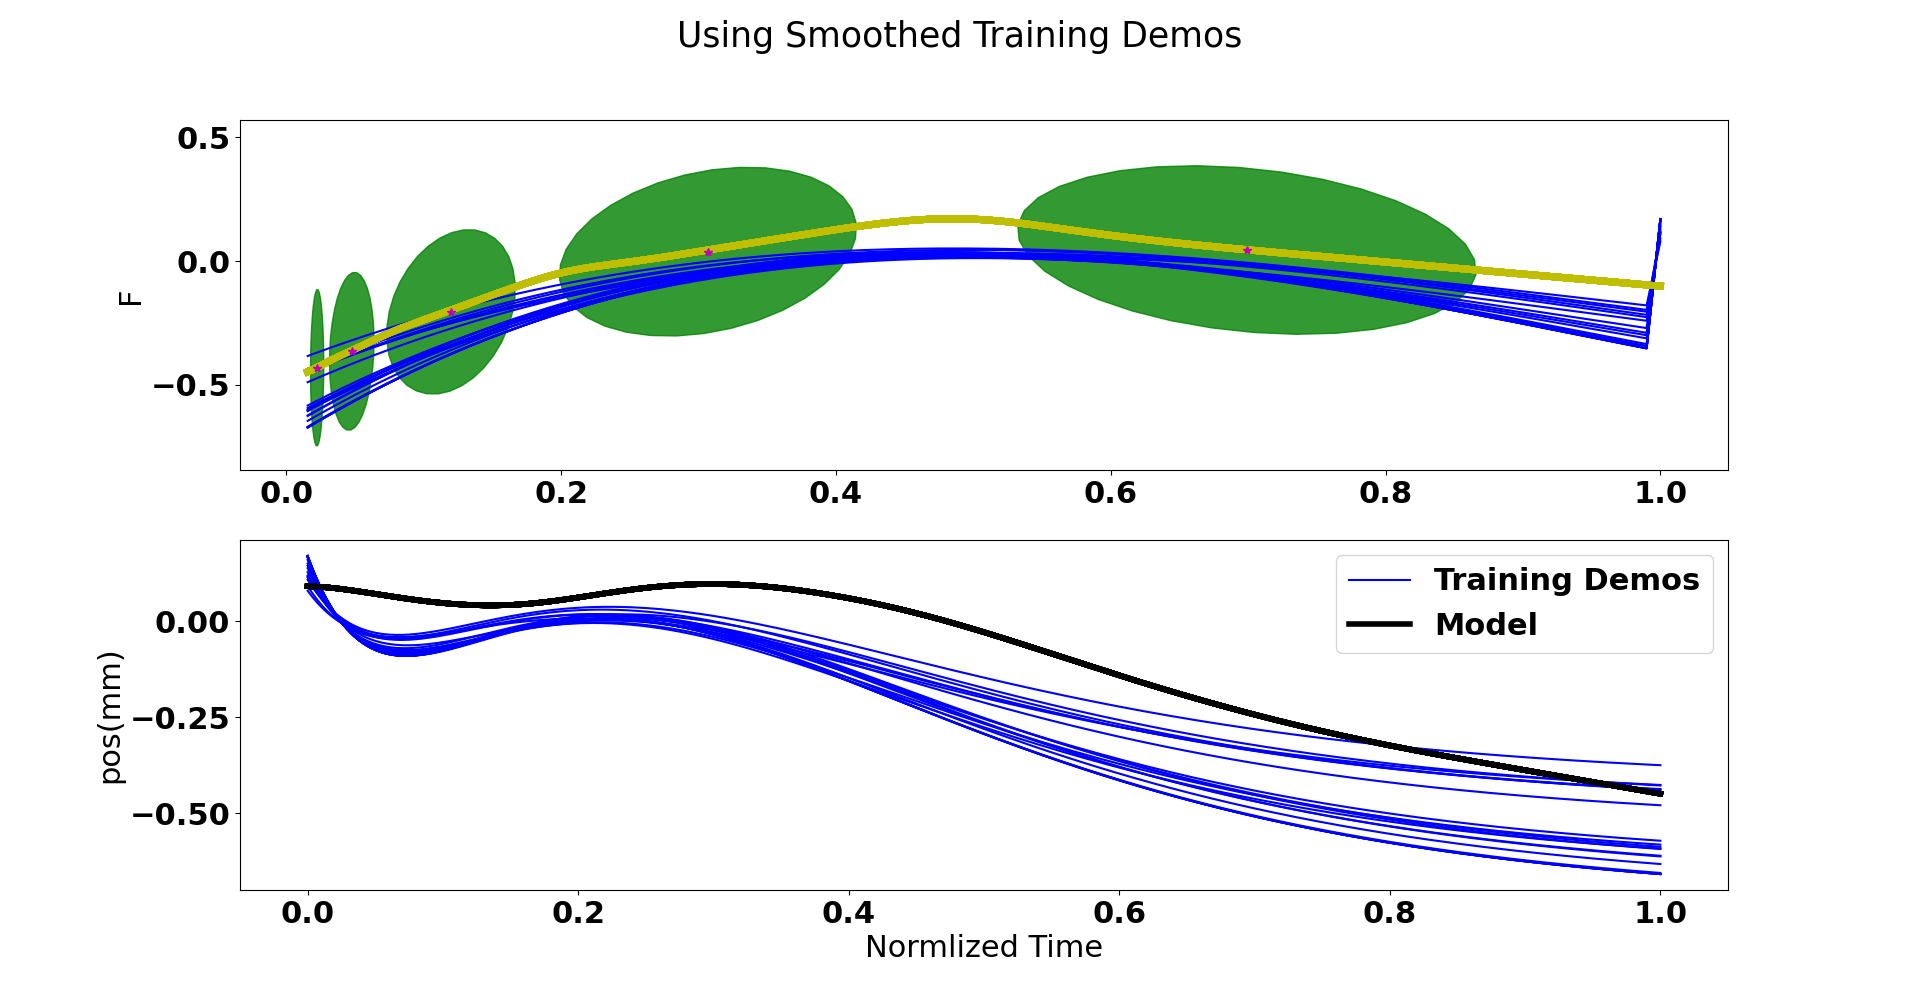
\includegraphics[width=\textwidth]{images/software/smoothed_repruction.png}
        \caption{Forcing function and replicated trajectory. As shown the model was able to follow the desired motion and the forcing functions are smooth along the motion.}
        \label{fig:smoothreplication}
    \end{subfigure}
    \caption[DTW Smoothing]{Effects of applying smoothing the a DTW demonstration}
    \label{fig:smoothingcomparison}
\end{figure}


The Gait Analysis package takes a different approach by providing the tools to parse data and build the data structures. The user only has to provide the data set and basic understanding of Python. Another advantage of the approach is the separation of the learning and replication systems. As discussed in \autoref{sec:lfd} the learning phase is an offline process. Using GMM to encode a data set can take several seconds to several minutes depending on the number of demonstrations, length of the demonstrations, and the number of bins used to encode; this makes it desirable to use a powerful computer to encode the demonstrations. The replication of the trajectory with GMR is an online process using the parameters calculated by GMM. 

This separation of layers allows for the demonstrations to be learned once then can be played back later. The object-oriented approach reduces the amount of redundant code required. The package divides the tools into three parts allowing for additional algorithms to be developed and use the underlying structure: 

\begin{itemize}[noitemsep]
    \item \textbf{Model:} The main body of the algorithm, all the functions for handling the data. Examples of Models include (Gaussian Mixed Models(GMM), Gaussian Mixed Regression (GMR), Dynamics Motion Primitives (DMP), Task-Parameterized Gaussian Mixed Models (TPGMM). All of the Models extend the ModelBase class. This parent class contains properties and common functions to make it easy for future development.
    \item \textbf{Trainer:} This class handles the process of organizing and processing the data. The trainer's classes extend the base TrainerBase class, which has core functionality to parse and save the data. The trainer class will handle all the alignment and put the data in the model's proper form. The trainer pickles \footnote{https://docs.python.org/3/library/pickle.html} the parameters to be used later without needing to retrain the model. 
    \item \textbf{Runner:} The runner class reproduces the imitation model. The input to the model is the pickle file generated by the trainer. All the runners extend the RunnerBase class. This running method allows for feedback into the system. 
\end{itemize}


\section{Contributions}

The software packages presented have been released open-source for community use and development. The packages can be installed using pip for ease of use. The modularity of the packages allows for the underlying tools to be used to build parsers for other mocap systems like the OptiTrack \footnote{https://optitrack.com/} mocap system. The Vicon Toolkit Package parses and provides convenient tools for accessing and manipulating the mocap data. This package includes access to the raw marker position and allows for the manipulation of rigid body transformations. The Gait Analysis Toolkit provides tools for gait analysis independent Vicon package. It contains a tool for extracting cycles, gait comparison, EMGs analysis, and learning and comparing trajectories. The contributions of the packages are the following:

\begin{itemize}
    \item Open Source tools for handling mocap data.
    \item Improved methods to handle and analyze marker and rigid body data by allowing rigid bodies to be defined and automatically finding transformation between different bodies in every frame.
    \iten Visualization tools to observe the marker position and calculated joint centers. 
    \item Improved GMM process by introducing a polynomial smoothing function on the demonstrations to ensure smooth and differentiable. Doing this reduces the chattering in the forcing function used to train and drive the model along the desired trajectory; this was shown to reduce the metric of imitation.
    \item Comprehensive tools for learning from demonstrations to encode and reproduce biological motion. The encoding method is separated from the reproduction method allowing for offline learning and online reproduction.
    \item Modular method to fill in missing marker gaps, allowing different gap-filling methods to be implemented. 
    \item Built-in tools to parse and compare gait trajectories. 
    \item APIs provide access to the lower and upper body plug-in Vicon models. 
\end{itemize}

All of the toolkits presented here were built to handle all the collected human demonstration data in \autoref{chap:gaitdata}, this allowed for the gait cycles to be extracted and compared. The collected data was easily encoded using the built-in LfD tools. The separation of the layers allows the trajectories to be learned offline and replicated online. This feature was used to build the simulation of the exoskeleton in \autoref{chap:sim}.

